\section{Pwnfish Challenge}\label{sec:pwn-challenge}

\subsection{Challenge Overview}

% Every open challenge should be described providing the challenge name, a description of the challenge scenario, where the idea comes from, what participants need to accomplish (i.e., what skill is tested, the goal of the challenge) and the expected level of difficulty. In particular, you should also mention who was the primary proponent of the challenge, who was the primary developer and who else had a secondary role in the design/implementation of the challenge.

The "Pwnfish" challenge is a relatively standard example of a binary exploitation challenge. The purpose of the challenge is to illustrate some of the perils of C programming, as well as to gain a deeper understanding of how programs are executed on modern computers. % illustrate consequences of bad C programming?
% pitfalls that arise when programming in a low level language such as C.
The challenge revolves around a simple menu-based fishing game written in C. 
% To complete the challenge, participants must exploit a buffer overflow and format string vulnerability to circumvent protections compiled into the binary, and eventually spawn a shell to retrieve the flag.
As is typical of PWN challenges, the participant is provided with the compiled \code{pwnfish} program, which is also playable on a remote server. The handout also includes the source code and the version of the GNU C library (glibc)\cite{glibc} being used on the remote server (version 2.35). Once the player has crafted an exploit that works locally, they can execute it on the remote server to obtain the flag. 
% It is a simple menu based program, allowing the user to catch random fish and name them. The user can also display ASCII art of their fish, as well as release them. 
To complete the challenge, participants must exploit a buffer overflow and format string vulnerability to circumvent protections compiled into the binary, and eventually spawn a shell to retrieve the flag.
The motivation behind this challenge, was to explore how common security measures, such as PIE, ASLR and stack canaries, can be bypassed using well known exploitation techniques. We expect this challenge to be of a medium to hard difficulty, as it involves many intricate technical details.
% We want to illustrate that even with simple techniques such as buffer overflow, it is still possible to exploit programs that are compiled with standard security protections enabled. 

Tobias was the primary proponent and developer of the challenge, while the rest of the group contributed by testing and commenting on the challenge. 

\subsection{Technical Details}

% Provide a detail description of the implementation of the challenges including:
% \begin{itemize}
% 	\item Challenge Design: Step-by-step explanation of how the challenge works, including potential vulnerabilities, know how, or weaknesses that participants are expected to exploit. If possible use an image to illustrate the challenge architecture and how the different components interact.
% 	\item Environment and implementation: Describe the setup required (e.g., server configurations, programming language used, ...) and how the challenge was implemented.

%     64-bit x86
%     linux, glibc version 2.35, gcc version 11.4.0,
%     c standard = c11.
% 	\item Tools and Resources: Any tools or libraries used for creating the challenge.
% 	\item Difficulties Encountered: Describe any technical or conceptual challenges the group faced while creating this challenge.
% 	\item Design Choices: Explain why certain design decisions were made (e.g., complexity level, choice of vulnerability, tools used).
% 	\item Testing Process: How the challenge was tested to ensure it works as intended.

%         Valgrind to confirm memory is freed correctly.
%         Manual tests?
%         automated tests?
%         Tests by other people in group.
%         challenge id: 30e38171-ac1c-4e27-8c71-f609e0884535
        
% 	\item Difficulty Assessment: Rate and justify the challenge’s difficulty level.

%         We rate this challenge as a medium difficulty challenge. It requires a solid understanding of how programs are executed at a low level, and how to circumvent various protections against low level attack. Furthermore, it requires the player to be comfortable with tools such as gdb to inspect the memory during execution, and pwntools for crafting a complete exploit. There is, however no need to have knowledge of how the glibc allocator works, as the challenge does not require heap exploitation, so it is not among the hardest binary exploitation challenges.
%         Excluding the source code from the handout could also make the challenge slightly harder, encouraging the players to decompile the binary using e.g. Ghidra. This would make the scenario slight more realistic, but also when solving the challenge.
% The difficulty will depend heavily on the experience level of the participants. If the participant has no experience in the category, the challenge could be rather difficult, as it involves a wide array of concepts that may be unfamiliar. It does, however, not involve complex heap exploitation which requires deep understanding of glibc allocator in order to exploit\footcite{https://sourceware.org/glibc/wiki/MallocInternals}.
% \end{itemize}


\subsubsection{Architecture}
The architecture of this challenge is illustrated in Figure \ref{fig:pwnfish-architecture}. The structure is almost identical to that of the Maze Game challenge from section \ref{sec:maze-challenge}.
\begin{figure}[H]
    \centering
    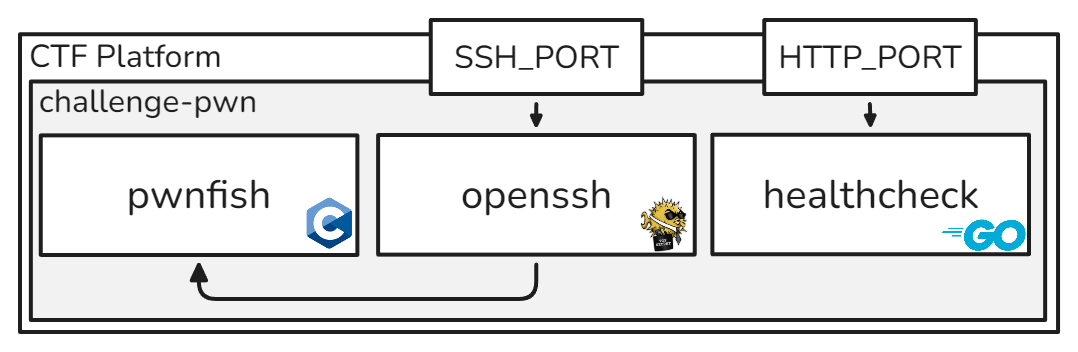
\includegraphics[width=0.85\linewidth]{img/challenge-pwn--architecture.png}
    \caption{Pwnfish challenge architecture}
    \label{fig:pwnfish-architecture}
\end{figure}
\noindent
As in the previous challenges, the OpenSSH server is used to facilitate access to the challenge environment, allowing participants to enter through SSH, and then connect to the \code{pwnfish} container (using e.g. netcat or pwntools). 
We also use a prebuilt image \code{cybersecnatlab/challenge-jail}\cite{challenge-jail} for the \code{pwnfish} challenge container shown in the figure, which allows for convenient and hardened setup of PWN challenges. The image was also used in the openECSC-2024 CTF competition\cite{openECSC}, which demonstrates its reliability. The image uses \code{nsjail}\cite{nsjail} to isolate the challenge even further, and \code{socaz}\cite{socaz} as the TCP forking server. Using this image allowed us to focus on the more technical details of the actual exploitation, while still ensuring that the challenge runs in a hardened environment.

\subsubsection{Challenge Design}
In this section, we begin to describe and justify the overall challenge design.
The \code{pwnfish} executable is compiled for the x86-64 architecture\cite{x86-64} from source files \code{main.c} and \code{fish\_t.h}, with standard protections applied by the GNU C compiler (gcc)\cite{gcc} version 11.4.0 on Ubuntu 22.04.5 LTS. These protections are explicitly enabled with flags in the Makefile in appendix \ref{apx:pwnfish-makefile}, though they would be enabled by default on most systems\footnote{The Makefile in the verified challenge does not have the flags explicitly enabled. However, inspecting the binary with \code{checksec} confirms that they have been applied.}.
% The \code{fish\_t.h} file contains a type \code{fish\_t} used to represent fish, as well as some ASCII art for the three species, while the main logic is found in \code{main.c}. 
The program provides a simple menu with five options as an interface to the user. The user can catch and name a new pet fish, which is then added to a singly-linked list on the heap containing all fish. The user can choose to show a fish with a specific name, and the program then prints the fish. The user can also list the names of all caught fish, and release a fish with a specific name. Finally, the user may exit the program safely.

We designed and implemented the challenge in a highly iterative manner, starting with a simple buffer overflow and no protections enabled. We ended with a program that has all default protections enabled, which was the ambition.

Since we use the heap to store the linked list of fish, it would be very natural to iterate on the challenge in the future to require heap-based exploitation techniques instead of the current stack-based vulnerabilities. This would make the challenge even harder and the vulnerabilities more realistic.

Another consideration is whether to include the source code in the handout. Excluding the source code from the handout could make the challenge slightly harder, encouraging the participants to decompile the binary using a decompiler such as Ghidra\cite{ghidra}. This would make the scenario slightly more realistic, but also introduce more friction for participants solving the challenge. We chose to include the source code, so the participants can focus on the main exploitation techniques, which makes the challenge somewhat less challenging.

\subsubsection{Vulnerabilities and Protections}
In the following section, we aim to explain and justify the main vulnerabilities and protections present. 
% The actual implementation details the  are not very interesting apart from the deliberate vulnerabilities, and we therefore only focus on these exploitable parts.
The first vulnerability comes from using \code{scanf("\%s", buffer)} to get user input. When using \code{scanf} in this way, there is no limit on the length of the input; the function only stops reading when it encounters a whitespace character. Thus, if reading into a buffer on the stack, it is possible to overflow the buffer and overwrite values, such as the stored instruction pointer at the bottom of the current stack frame. Appendix \ref{apx:show_fish} contains the \code{show\_fish} function, which misuses \code{scanf} as described. The \code{scanf} function, which, while highly dangerous, reflects a more realistic programming error than the use of the deprecated \code{gets} function. The compiler explicitly warns about the use of some dangerous functions such as \code{gets}, but gives no warning when using \code{scanf("\%s", buffer)} since there are correct ways to use \code{scanf}, while \code{gets} is deprecated and should never be used. Therefore, using \code{scanf} is still a potential pitfall for inexperienced programmers. 
A technique commonly used with buffer overflows is return-oriented programming (ROP)\cite{rop}. This type of attack chains small pieces of code together, called gadgets, that all end with a \code{ret} instruction. This is accomplished by putting the addresses of the gadgets on the stack in order beginning at the stored instruction pointer. Using a ROP chain, it is possible to string together an fairly complex series of instructions, and eventually spawn a shell.


% The first vulnerability is the use of \code{scanf} for taking user input. The \code{scanf} function is not inherently dangerous, but when naively using \code{scanf("\%s", buffer)} to get a string as input, there is no limit on the number of bytes read from stdin; the function only stops reading when encountering a whitespace character, thus allowing for a buffer overflow attack on the stack. The safe approach would be to limit the input length, which is possible with \code{scanf}, but \code{fgets} is usually more convenient to use. We have chosen to use \code{scanf} everywhere a string is taken as input, simulating a situation where the developer is unaware of the danger, and thus keeping the scheme consistent, though one could argue that only using it in one place makes the intended exploit more clear. Figure \ref{fig:show-fish} contains the \code{show\_fish} function.
% \todo{code snippet?}

% The misuse of \code{printf} format strings is another vulnerability. Calling \code{printf(name)} seems innocent at first glance, but the first argument to \code{printf} can contain format specifiers that are used to print dynamic arguments. If \code{name} buffer is controlled by user input, the user can, for example, provide \code{"\%4\$p"} as input. The \code{printf} will consequently find the format specifier and then try to read the fourth argument to the function and print it as a pointer. Since no extra arguments were passed to \code{printf}, it will simply expect that another argument was provided, and print from the location arguments are usually store. In this case, the values printed in order are stored in the \code{rsi}, \code{rdx}, \code{rcx}, \code{r8}, and \code{r9} registers, and the rest will be read off the top of the stack. This is due to the x86-64 system V ABI calling convention\footcite{https://wiki.osdev.org/Calling_Conventions##System_V_ABI}.


% It will first read the values stored in the registers rsi, rdx, rcx, r8, and r9, and then read additional values off the top of the stack as specified in the x86-64 system V ABI calling convention\footcite{https://wiki.osdev.org/Calling_Conventions##System_V_ABI}.

The other vulnerability comes from using \code{printf} format strings incorrectly. The vulnerability is present on line 10 in the \code{show\_fish} function with \code{printf(curr->name)}. This naive use of \code{printf} gives the user control of the first argument, which may contain format specifiers such as \code{\%p} or \code{\%s}. Only one argument was passed to \code{printf}, but if the first argument contains format specifiers, \code{printf} will expect more arguments, and try to access them. Now, arguments are passed to functions through specific registers, as well as the stack, as defined by the x86-64 System V ABI\cite{systemv}. It is therefore possible to print arbitrary values from the stack by passing format specifiers such as \code{\%8\$p} to leak the 8th argument, which is extremely useful in bypassing stack canaries and ASLR.
The \code{\%s} format specifier is even more powerful, and will take an address on the stack and print the string stored at that address. If part of the stack contains user input, it becomes possible to read arbitrary memory locations. The format string vulnerability triggers an explicit warning by the compiler (unless \code{-Wno-format-security} is enabled), and is therefore less realistic to appear in modern programs, but is it still interesting how it can be used to bypass protections. It is a versatile and powerful exploit, while being fairly simple. Hence, it is particularly well suited to demonstrating how protections can be bypassed

Next, we describe the protections compiled into the binary, and how a user can exploit the vulnerabilities to bypass them. 
There are a few protections enabled to prevent the simplest exploits. The first protection is no execution (NX) of stack memory. This protects against simple buffer overflows that simply inject shellcode onto the stack, and then overwrites the old instruction pointer to point back at the shellcode. Relocation Read-Only (RELRO)\cite{relro} is used to protect the Global Offset Table (GOT)\cite{got} from simply being overwritten by the format string exploit.
% The first protection is no execution (NX) of the stack memory. This protects against buffer overflow attacks that inject a series of instructions that spawn a shell, typically called shellcode.
% by invoking the \code{execve} syscall.
% The buffer overflow allows the attacker to overwrite the stored instruction pointer on the stack, so when the current function returns, the can redirect execution to the shellcode.
% The no-execute NX bit
% Passing \code{-z noexecstack} tells the linker to mark the binary with no execution of stack memory, which is enforced if the hardware/operating system supports it \todo{it does}. This prevents certain buffer overflow attacks, that inject shellcode onto the stack, and the overwrite the store return pointer to jump to the shellcode on the stack. The shellcode is just a short series of instructions that changes

% set marks the binary with the NX-bit enabled

The binary is a Position-Independent Executable (PIE)\cite{pie}, which affects the static data and code addresses in the binary. 
As a result, each address is relative instead of being absolute, and is defined with an offset from the base. The program can then be loaded with a different base address every time it is executed. 
% Addresses in the binary are defined only in terms of offsets, and it is loaded at a different base address each time. 
This makes ROP based attacks much harder, since one cannot rely on hardcoded static addresses.
To ensure the program uses a different PIE base address every time it is executed, it is crucial that address space layout randomization (ASLR)\cite{aslr} is be enabled. ASLR is an operating system security feature and is enabled by default on the challenge VM. ASLR partially randomizes the base addresses of the different memory regions in a process. This also affects the base address of dynamically linked libraries such as glibc. This protection makes the challenge much more interesting to solve, as the participant needs to cleverly leak addresses with known relative offsets from the binary and glibc, in order to calculate the base addresses.

Another hardening strategy is stack canaries, which are random values placed on the stack at the beginning of a function to protect from buffer overflow attacks\cite{canary}. Before the function returns it will check the stack canary for modifications, and crash if it has changed. Consequently, a buffer overflow that overwrites the canary will cause the program to crash. The stack canary can be bypassed with the format string exploit, since it can leak the canary from the stack.
% which is enabled in gcc by default in recent versions of Ubuntu ($\geq 14.10$) with \code{-fstack-protector-strong}\footcite{https://manpages.ubuntu.com/manpages/jammy/en/man1/gcc.1.html}. 
% since it is enabled by default in Ubuntu \code{-fstack-protector-strong}. 
% is a security measure compiled into the binary, that can be enabled with .




\subsubsection{Solution}
The solution script \texttt{solve.py} (Appendix \ref{apx:pwnfish-solve}) contains the most interesting implementations details of the challenge. We used \code{gdb}\cite{gdb} with the \code{pwndbg}\cite{pwndbg} plug-in to analyze the binary during execution, and inspect various address-offsets required for the solver. To start, the solution script uses \code{sshtunnel}\cite{sshtunnel} to tunnel through the OpenSSH server, using username "gl" and password "hf". The script then uses \code{pwntools}\cite{github__pwntools} to access the challenge remotely. The concrete steps are then as follows:
\begin{itemize}
    \item Use the format string exploit to leak the stack canary.
    \item Leak the address of a known instruction in the binary (in this case an address in the \code{menu} function) from the stack and use it to compute the PIE base address.
    \item Leak the address of the \code{puts} function from the GOT, and use it to compute the base address of glibc.
    \item Find the addresses of the \code{system} function and the string \code{"/bin/sh"} in glibc.
    \item Find the addresses of ROP gadgets for \code{pop rdi} and \code{ret}.
    \item Construct a payload with a ROP chain to call \code{system("/bin/sh")} which spawns a shell.
    \item Read the flag with \code{"cat flag"} and write it to \code{/run/solution/flag.txt}.
\end{itemize}
We encountered various difficulties while developing the solver. 
One problem was that \code{scanf} only reads until the first whitespace byte, which is a problem if an address in a payload happens to contain a whitespace byte. If this happens, the exploit will fail, since the payload is only read partially. Therefore, the solver works probabilistically, and retries if a payload contains a whitespace byte, trying at most 20 times before failing\footnote{Experimentally, we found that the exploit succeeds approximately 50\% of the time. Consequently, the probability of all 20 attempts failing is roughly one in a million, which we consider to be acceptable.}.

% \todo{Probably remove this idk}
% Experimentally, we found that the exploit succeeds around half the time, so trying 20 times results in roughly a $1/2^{20}$ chance of failure. In other words, we expect the solver to fail with a probability of roughly one in a million, which we believe is acceptable.

Another interesting problem is stack alignment. The x86-64 System V ABI\cite{systemv} guarantees that the stack is 16-byte aligned before a function call. The \code{system} function relies on this assumption for certain instructions such as \code{movaps}. Therefore, there is an extra \code{ret} gadget in the final ROP payload, which aligns the stack for \code{system}.

% DIFFICULTIES encountered

% \code{scanf} only reads until a whitespace character is encountered, so if an address in the payloads happens to contain a whitespace byte only part of the payload is read, and the exploit will fail. Therefore, the solver works probabilistically, and may have to retry the exploit a few times. During testing we found that it usually requires no more than four tries for the solver to succeed. Therefore, it tries 20 times, so if it succeeds half of the time, the probability of failing all 20 times is around one in a million.
% \todo{Change number of tries?}
% it is vanishingly unlikely to fail all tries.

% \subsubsection{Design Choices}
% • Design Choices: Explain why certain design decisions were made (e.g., complexity
% level, choice of vulnerability, tools used).
% We designed and implemented the challenge in a highly iterative manner, starting with a simple buffer overflow and no protections enabled. Then, and ending with a program that has all default protections enabled, which was the ambition.

% Since we use the heap to store the linked list of fish, it would be very natural to iterate on the challenge in the future to require heap-based exploitation techniques instead of the current vulnerabilities. This would make the challenge even harder and the vulnerabilities more realistic.

% Another consideration is whether to include the source code in the handout. Excluding the source code from the handout could also make the challenge slightly harder, encouraging the players to decompile the binary using a decompiler such as Ghidra\cite{ghidra}. This would make the scenario slight more realistic, but also introduce more friction for participants solving the challenge. We chose to include the source code, so the participants can focus on the main exploitation techniques, making the challenge slightly easier.

\subsubsection{Testing}
We tested the challenge manually both locally and on the CTF platform, and confirmed that the challenge appears to function as intended. These were not rigorous functionality tests, so there may be unintended vulnerabilities or errors present. Since the goal is to obtain a shell, any unintended solution is not likely to pose a greater threat compared to the intended solution. The challenge was also tested heavily with the automated solve script described above.
The challenge has been successfully verified on the CTF platform with challenge ID: \texttt{30e38171-ac1c-4e27-8c71-f609e0884535}.

\textbf{Note:} During the final stage of testing, just before submitting the project, we discovered a critical error in the automated solution script. This occurred well after the challenge was successfully verified, and prior to this point, the solution had worked without issue numerous times. The error is that the \code{system} function is found at offset \code{0x050d70} in glibc 2.35, which contains a whitespace byte, namely the carriage return byte: \code{0x0d}. Since the least significant bytes of this offset are unaffected by ASLR, the \code{scanf} function will always fail to read the whole payload. It is unclear why this only became an issue at the very end of the project, even using the exact same code that previously worked, since we used the same version of glibc throughout the whole development. This could potentially be fixed by using a different version of glibc with different offsets, or using a function that does not terminate on whitespace bytes to introduce the buffer overflow.


\subsubsection{Difficulty Assessment}
% The difficulty will depend heavily on the experience level of the participants. If the participant has no experience in the category, the challenge could be rather difficult, as it involves a wide array of concepts that may be unfamiliar. It does, however, not involve complex heap exploitation which requires deep understanding of glibc allocator in order to exploit.

We rate this challenge as a medium to hard difficulty challenge. It requires a solid understanding of how programs are executed at a low level, and how to circumvent various protections. Furthermore, it requires the player to be comfortable with tools such as \code{gdb} to inspect the memory during execution, and \code{pwntools} for crafting a complete exploit. There is, however, no need to have knowledge of how the glibc allocator works, as the challenge does not require heap exploitation, so it is not among the hardest binary exploitation challenges\cite{malloc}. The source code and glibc version are also included, streamlining the exploitation process, and thus making the challenge slightly easier.



% NOTES:

% The compiler warns about the use of dangerous functions such as \code{gets}, but gives no warning when using \code{scanf("\%s", buffer)}. This is because there are correct ways to use the \code{scanf} function, while \code{gets} is deprecated and should never be employed. It is still a potential pitfall for inexperienced programmers. The format string vulnerability triggers an explicit warning by the compiler (unless \code{-Wno-format-security} is enabled), and is therefore less realistic in a real program.

% Standard security protections depends heavily on 
% gcc -v to see versions

% The handout includes the compiled binary, the corresponding source code and the glibc and linker used on the remote server

% buffer overflow could also be done in \code{release\_fish}.

% These are arguably fairly egregious mistakes - it is highly unlikely that an experienced developer will make mistakes that are this dangerous. In sufficiently large code bases however, it is conceivable and also documented \todo{source} that these vulnerabilities occur. A strong case can be made that the format string vulnerability is especially unrealistic since the compiler provides an explicit warning, though it would not be the first time a warning is ignored.

% Challenge hardening:
% nsjail
% TODO: limit memory consumption of containers.

% These security measures are all enabled by default when compiling in newer version of Ubuntu.


% https://hub.docker.com/r/cybersecnatlab/challenge-jail#configuration
% https://hub.docker.com/r/cybersecnatlab/socaz
% https://manpages.ubuntu.com/manpages/jammy/en/man8/ld.so.8.html
% https://sourceware.org/glibc/wiki/MallocInternals